%!TEX root = ../../thesis.tex

\chapter{مقدمه} \label{chapter:introduction}

محتوای فصل اول به صورت نمونه در خطوط زیر قرار گرفته است.

دانشگاه شهید چمران اهواز یک دانشگاه دولتی در کلان‌شهر اهواز، چهارمین دانشگاه بزرگ کشور و بزرگ‌ترین دانشگاه در جنوب ایران است. دانشگاه شهید چمران به دلیل امکانات گسترده و فضای آموزشی بسیار وسیع از معتبرترین دانشگاه‌های ایران می‌باشد. این دانشگاه با ۱۵ دانشکده و ۱ پردیس دانشگاهی، یکی از ۱۰ دانشگاه برتر جامع کشور محسوب می‌شود که در سال ۱۳۳۲ تأسیس شد. نام قدیم این دانشگاه جندی شاپور بوده‌است. مطابق ارزیابی‌های وزارت علوم، دانشگاه شهید چمران اهواز یکی از دانشگاه‌های «سطح یک» کشور به‌شمار می‌رود.
%==SECTION==%
\section{تاریخچه}\label{sec:history}

قدمت دانشگاه جندی‌شاپور، به سدهٔ چهارم یا پنجم میلادی بازمی‌گردد و در طی ۶ قرن، نام جندی‌شاپور مترادف با مرکزی علمی در رشته‌های مختلف بوده‌است و عصر تعالی و ترقی آن در زمان خسرو انوشیروان بوده‌است. مکان شهر دانشگاهی جندی‌شاپور در دوران ایران باستان به‌طور قطعی مشخص نیست، اما به گفته احمد اقتداری از منابع گوناگون برمی‌آید که در محدوده میان شهرهای شوشتر، شوش و دزفول قرار داشته‌است.\cite{eghtedari00diyar}

دانشگاهی با نام گندی‌شاپور در یکشنبه ۲ مهر ماه سال ۱۳۳۴ در اهواز گشایش یافت. پس از چندی این نام به جندی‌شاپور تغییر کرد. دانشگاه در نزدیکی رودخانهٔ کارون، در زمینی هموار و نزدیک باغ گیاهان گرمسیری بنا گردید. به دلیل طراحی چندین بنا و دانشکده توسط معمارانی نظیر کامران دیبا و آندره گدار، ساختمان این دانشگاه، از معماری منحصر به فردی برخوردار است.

مرجع \cite{Omidali82phdThesis} یک نمونه پروژه دکترا و مرجع \cite{Vahedi87} یک نمونه مقاله مجله فارسی است.
مرجع \cite{Amintoosi87afzayesh}  یک نمونه  مقاله کنفرانس فارسی و
مرجع \cite{Pedram80osool} یک نمونه کتاب فارسی با ذکر مترجمان و ویراستاران فارسی است. مرجع \cite{Khalighi07MscThesis} یک نمونه پروژه کارشناسی ارشد انگلیسی و
\cite{Khalighi87xepersian} هم یک نمونه متفرقه  می‌باشند.

مرجع \cite{Gonzalez02book} یک نمونه کتاب لاتین است که از آنجا که دارای فیلد \lr{authorfa} است، نام نویسندگان آن در استیلهای \lr{asa-fa}، \lr{plainnat-fa} و \lr{chicago-fa} به فارسی دیده می‌شود. مرجع \cite{Baker02limits} مقاله انگلیسی است که معادل فارسی نام نویسندگان آن ذکر نشده بوده است.



%==SUBSECTION==%
\subsection{معادله ریاضی}\label{sec:math-equation}
نمونه یک فرمول ریاضی در لاتک را در خطوط بعدی مشاهده خواهید کرد:

\begin{equation}
	\label{eq:a}
    J(\theta)=\frac{1}{2 m} \sum\left(h_{\theta}\left(x^{(i)}\right)-y^{(i)}\right)^{2}
\end{equation}

%==SUBSECTION==%
\subsection{تصویر نمونه}\label{sec:sample-image}
یک تصویر نمونه را در لاتک مشاهده می‌کنید.

\begin{figure}[H]
    \label{fig:main-gate}
    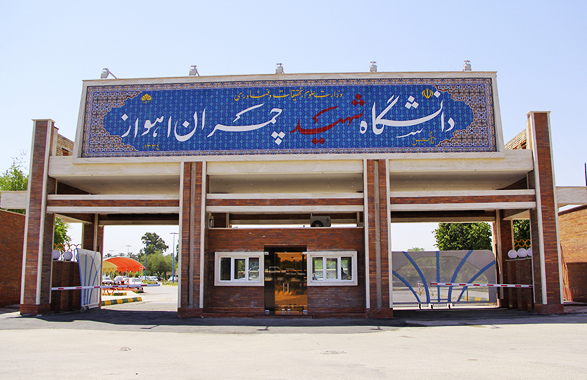
\includegraphics[width=0.5\textwidth]{chapter01/scu_main_gate}
    \caption{سردر غربی دانشگاه چمران}
\end{figure}

\subsection{تصویر چندتایی}\label{sec:multi-image}
\begin{figure}[H]
	\begin{subfigure}[t]{5cm}
		\centering
		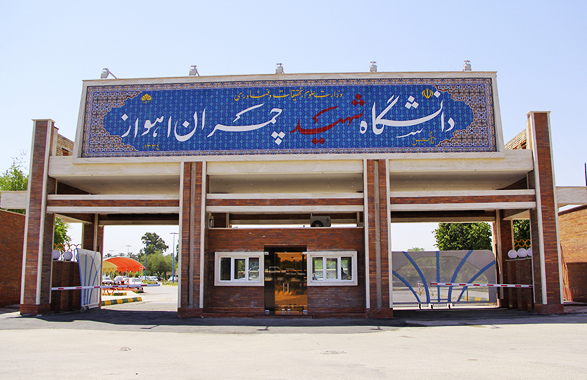
\includegraphics[width=5cm]{chapter01/scu_main_gate}
		\caption{ورودی شمالی}\label{fig:1a}		
	\end{subfigure}
	\quad
	\begin{subfigure}[t]{5cm}
		\centering
		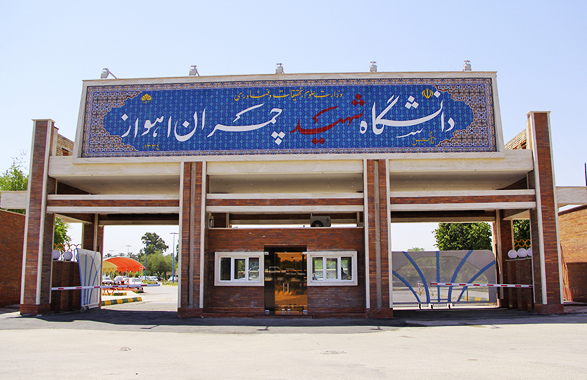
\includegraphics[width=5cm]{chapter01/scu_main_gate}
		\caption{ورودی جنوبی}\label{fig:1b}
	\end{subfigure}
	\caption{ورودی‌های دانشگاه چمران}\label{fig:1}
\end{figure}


\section{نمودار}

\begin{figure}[H]
	\begin{tikzpicture}
		\begin{loglogaxis}[
			xlabel=هزینه,
			ylabel=خطا]
		\addplot coordinates {
			(5,     8.31160034e-02)
			(17,    2.54685628e-02)
			(49,    7.40715288e-03)
			(129,   2.10192154e-03)
			(321,   5.87352989e-04)
			(769,   1.62269942e-04)
			(1793, 4.44248889e-05)
			(4097, 1.20714122e-05)
			(9217, 3.26101452e-06)
		};
		\addplot plot coordinates {
			(7,     8.47178381e-02)
			(31,    3.04409349e-02)
			(111,   1.02214539e-02)
			(351,   3.30346265e-03)
			(1023,  1.03886535e-03)
			(2815,  3.19646457e-04)
			(7423,  9.65789766e-05)
			(18943, 2.87339125e-05)
			(47103, 8.43749881e-06)
		};
		\legend{\rl{حالت ۱},\rl{حالت ۲}}
		\end{loglogaxis}
	\end{tikzpicture}
	\caption{مثال}
\end{figure}

\subsection{رسم انتگرال یک تابع}\label{sec:math-plot}
\begin{figure}[H]
    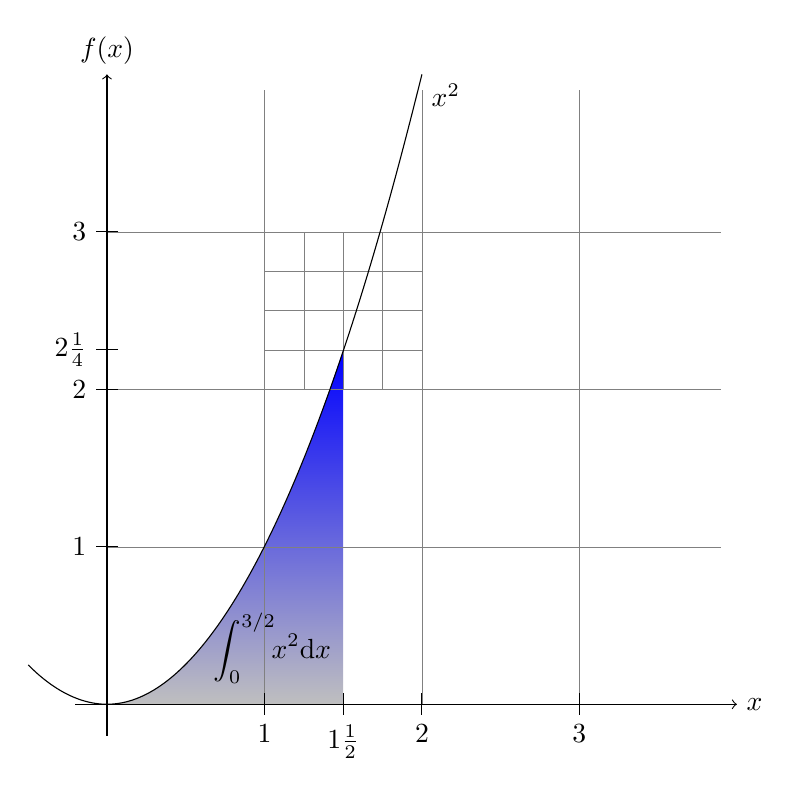
\begin{tikzpicture}[scale=2]
        \shade[top color=blue,bottom color=gray!50] 
            (0,0) parabola (1.5,2.25) |- (0,0);
        \draw (1.05cm,2pt) node[above] 
            {$\displaystyle\int_0^{3/2} \!\!x^2\mathrm{d}x$};

        \draw[style=help lines] (0,0) grid (3.9,3.9)
                [step=0.25cm]      (1,2) grid +(1,1);

        \draw[->] (-0.2,0) -- (4,0) node[right] {$x$};
        \draw[->] (0,-0.2) -- (0,4) node[above] {$f(x)$};

        \foreach \x/\xtext in {1/1, 1.5/1\frac{1}{2}, 2/2, 3/3}
            \draw[shift={(\x,0)}] (0pt,2pt) -- (0pt,-2pt) node[below] {$\xtext$};

        \foreach \y/\ytext in {1/1, 2/2, 2.25/2\frac{1}{4}, 3/3}
            \draw[shift={(0,\y)}] (2pt,0pt) -- (-2pt,0pt) node[left] {$\ytext$};

        \draw (-.5,.25) parabola bend (0,0) (2,4) node[below right] {$x^2$};
    \end{tikzpicture}
\end{figure}

\section{علائم و اختصارات}

مثلا \gls{optimizer}
مثلا \gls{kernel}
مثلا \gls{mse}
مثلا \gls{cnn}
